
%% bare_conf.tex
%% V1.4
%% 2012/12/27
%% by Michael Shell
%% See:
%% http://www.michaelshell.org/
%% for current contact information.
%%
%% This is a skeleton file demonstrating the use of IEEEtran.cls
%% (requires IEEEtran.cls version 1.8 or later) with an IEEE conference paper.
%%
%% Support sites:
%% http://www.michaelshell.org/tex/ieeetran/
%% http://www.ctan.org/tex-archive/macros/latex/contrib/IEEEtran/
%% and
%% http://www.ieee.org/

%%*************************************************************************
%% Legal Notice:
%% This code is offered as-is without any warranty either expressed or
%% implied; without even the implied warranty of MERCHANTABILITY or
%% FITNESS FOR A PARTICULAR PURPOSE! 
%% User assumes all risk.
%% In no event shall IEEE or any contributor to this code be liable for
%% any damages or losses, including, but not limited to, incidental,
%% consequential, or any other damages, resulting from the use or misuse
%% of any information contained here.
%%
%% All comments are the opinions of their respective authors and are not
%% necessarily endorsed by the IEEE.
%%
%% This work is distributed under the LaTeX Project Public License (LPPL)
%% ( http://www.latex-project.org/ ) version 1.3, and may be freely used,
%% distributed and modified. A copy of the LPPL, version 1.3, is included
%% in the base LaTeX documentation of all distributions of LaTeX released
%% 2003/12/01 or later.
%% Retain all contribution notices and credits.
%% ** Modified files should be clearly indicated as such, including  **
%% ** renaming them and changing author support contact information. **
%%
%% File list of work: IEEEtran.cls, IEEEtran_HOWTO.pdf, bare_adv.tex,
%%                    bare_conf.tex, bare_jrnl.tex, bare_jrnl_compsoc.tex,
%%                    bare_jrnl_transmag.tex
%%*************************************************************************

\documentclass[conference,reqno]{IEEEtran}

\usepackage{graphicx}
\graphicspath{{images/}}

\usepackage{amssymb}
\usepackage{amsmath}
\usepackage{adjustbox}
\usepackage{url}
% url.sty was written by Donald Arseneau. It provides better support for
% handling and breaking URLs. url.sty is already installed on most LaTeX
% systems. The latest version and documentation can be obtained at:
% http://www.ctan.org/tex-archive/macros/latex/contrib/url/
% Basically, \url{my_url_here}.

% correct bad hyphenation here
\hyphenation{op-tical net-works semi-conduc-tor}

\begin{document}

\title{UGAN: Underwater Image Restoration using Generative Adversarial Networks}

\author{\IEEEauthorblockN{Cameron Fabbri}
\IEEEauthorblockA{Information Directorate\\
Air Force Research Laboratory \\
Rome, NY, USA.\\
cameron.fabbri@us.af.mil}
\and
\IEEEauthorblockN{Md Jahidul Muslim}
\IEEEauthorblockA{UMN\\}
\and
\IEEEauthorblockN{Junaed Sattar}
\IEEEauthorblockA{UMN\\
}}

% for over three affiliations, or if they all won't fit within the width
% of the page, use this alternative format:
% 
%\author{\IEEEauthorblockN{Michael Shell\IEEEauthorrefmark{1},
%Homer Simpson\IEEEauthorrefmark{2},
%James Kirk\IEEEauthorrefmark{3}, 
%Montgomery Scott\IEEEauthorrefmark{3} and
%Eldon Tyrell\IEEEauthorrefmark{4}}
%\IEEEauthorblockA{\IEEEauthorrefmark{1}School of Electrical and Computer Engineering\\
%Georgia Institute of Technology,
%Atlanta, Georgia 30332--0250\\ Email: see http://www.michaelshell.org/contact.html}
%\IEEEauthorblockA{\IEEEauthorrefmark{2}Twentieth Century Fox, Springfield, USA\\
%Email: homer@thesimpsons.com}
%\IEEEauthorblockA{\IEEEauthorrefmark{3}Starfleet Academy, San Francisco, California 96678-2391\\
%Telephone: (800) 555--1212, Fax: (888) 555--1212}
%\IEEEauthorblockA{\IEEEauthorrefmark{4}Tyrell Inc., 123 Replicant Street, Los Angeles, California 90210--4321}}

% make the title area
\maketitle

% As a general rule, do not put math, special symbols or citations
% in the abstract
\begin{abstract}
Autonomous underwater robots often rely on visual input for decision making due to its non-intrusive and passive nature.
However, due to many factors such as light refraction, particles in the water, and color distortion, images are often times very noisy.
This paper propose a method using Generative Adversarial Networks (GANs) to denoise underwater images, and show that these 
images provide both increased accuracy for an underwater tracking algorithm, as well as a more visually appealing image.
Furthermore, we show how recently proposed methods are able to generate a dataset for the purpose of underwater image reconstruction.
\end{abstract}

\IEEEpeerreviewmaketitle

\section{Introduction}
TODO - talk about having to go back to the same location if you want to get good/bad pairs of the "same" image.
Vision is a commonly used sensor in autonomous underwater robots due to its non-intrusive, passive, and energy
effecient nature. The monitoring of coral reefs \cite{shkurti2012multi}, deep ocean exploration
\cite{whitcomb2000advances}, and mapping of the seabed are all tasks suitable for autonomous robots because they
provide safety by taking the risk instead of a human. Despite the advantages vision provides, many underwater
environments can be quite noisy due to light refraction and particles present in the water. Because red wavelengths are
quickly absorbed by water, images tend to have a green or blue hue to them. As you go deeper, this worsens as more
and more red wavelengths are being absorbed. This extremely non-linear distortion has many factors such as the amount
of light present (overcast vs sunny or depth), particles in the water, time of day, and the camera being used. This may
cause difficulty in tasks such as segmentation, tracking, or classification due to their indirect or direct use of
color.

As color and illumination begin to change with the depth, vision based algorithms must be very generalizable in order
to work within the depth ranges a robot may operate in. Because of the high cost and difficulty of acquiring a
variety of underwater data, as well as the high amount of noise introduced, many algorithms may perform poorly in
these different domains. Figure 1 shows the high variability that may occur in underwater environments. A step towards a
solution to this
issue is to be able to restore the images such that they appear to be above water, i.e., with colors corrected and
particles removed. By performing a many to one mapping of these domains from underwater to not underwater (what the
image would look like in the air), algorithms that have

\begin{figure}[!htb]
   \begin{center}$
      \begin{array}{cccc}
         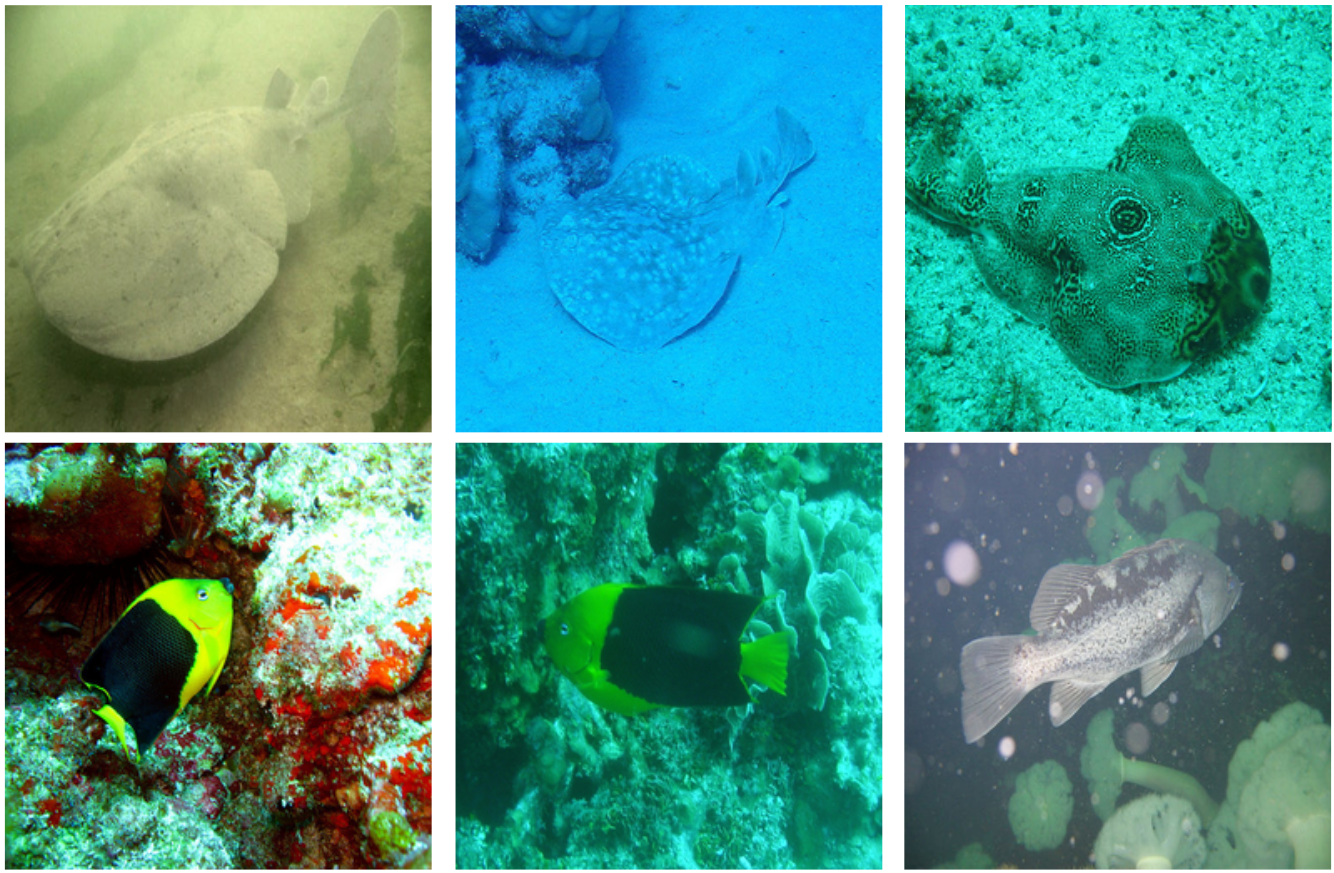
\includegraphics[width=3in]{figure1}
      \end{array}$
   \end{center}
   \caption{Underwater images showing the vast divesity of noise that can occur, including
   different hues of green and blue, as well as particles in the water.}
\end{figure}

\noindent difficulty performing across multiple forms of noise may be able to focus only one clean domain.

Deep neural networks have been shown to be powerful non-linear function approximators, especially in the field of
vision. Often times, these networks recquire large amounts of data, either labeled or paired with ground truth.
For the problem of automatically colorizing grayscale images, paired training data is essentially free due to the
fact that any color image can be converted to black and white. However, underwater images distorted by either color
or some other visual effect lack ground truth. We use the recently proposed CycleGAN \cite{zhu2017unpaired}, which
learns to translate an image from domain $X$ to domain $Y$, as a way to generate a paired dataset. By letting $X$ be
a set of undistorted underwater images, and $Y$ be a set of distorted underwater images, we can generate an image
that appears to be underwater while retaining ground truth.

\section{Related Work}

While there have been many very successful recent approaches towards automatic colorization
\cite{zhang2016colorful,iizuka2016let}, most are focused on the task of grayscale to color.
The work of \cite{torres2005color} used an energy minimization formulation using a Markov Random Field. 
MORE RELATED BLAH. Many use physics based models to directly model the light source and such.
Most similar to our line of work is the recently proposed WaterGAN \cite{li2017watergan}, which uses
GANs for color correction of underwater images. As ground truth pairs do not exist for underwater images,
their first step is to structure a generator to create realistic underwater images. Their generator model
can be broken down into three stages: 1) Attenuation, which accounts for range-dependent attenuation of light.
2) Scattering, which models the haze effect caused by photons scattering back towards the image sensor. 3)
Vingetting, which produces a shading effect on the image corners that can be caused by certain camera lenses.
Opposed to our work, they use a GAN for generating the underwater images and Euclidean loss for color correction,
where as we use a GAN for both. Furthermore, they require depth information during the training of WaterGAN,
whereas we only require two separate image domains.

Recent work in generative models, specifically GANs, have shown great success
in areas such as inpainting \cite{pathak2016context}, style transfer \cite{Gatys_2016_CVPR}, and image-to-image
translation \cite{isola2016image,zhu2017unpaired}. This is highly due to their ability to provide a more meaningful
loss than simply the Euclidean distance, which has been shown to produce blurry results. In our work, we structure
the problem as paired image-to-image translation, using Generative Adversarial Networks (GANs) as our generative model.
Much like the work of \cite{isola2016image}, we use image pairs from two domains an input and ground truth.

\section{Method}

\subsection{Dataset Generation}
Here we describe our dataset generation process. Depth, lighting conditions, camera
model, and location are all factors that affect the amount of distortion an underwater image undergoes. Under certain
conditions, it is possible that an underwater image may have very little distortion, or none at all.
We let $I^C$ be an underwater image with no distortion, and $I^D$
be the same image with distortion. Our goal is to learn the function $f: I^D \rightarrow I^C$. Becasue of the
difficulty of collecting underwater data, more often than not only $I^D$ or $I^C$ exist, but never both.

We use the recently proposed CycleGAN \cite{zhu2017unpaired} to generate $I^D$ from $I^C$, which gives us a paired
dataset of images. Given two datasets $X$ and $Y$, where $I^C \in X$ and $I^D \in Y$, CycleGAN learns a mapping
$F: X \rightarrow Y$. Figure 2 shows paired samples generated from CycleGAN. From this paired dataset we train a
generator $G$ to learn the function $f: I^D \rightarrow I^C$. It should be noted that during our data generation process,
CycleGAN simultaneously learns a mapping $G: Y \rightarrow X$, which is similar to $f$. In section IV we show a comparison with our method.

\subsection{Adversarial Networks}
GANs \cite{goodfellow2014generative} are a class of generative models based on game theory in which a generator
network competes against an adversary. Conditioned on an image $I^D$, the generator is trained to produce an \
image to try and fool the discriminator, which is trained to distinguish be between distorted and non-distorted
underwater images. In the original GAN formulation, the goal is to solve the minimax problem: \newline

\begin{figure}
\centering
\begin{tabular}{p{1.7cm} p{1.7cm} p{1.7cm} p{1.7cm}}
   
   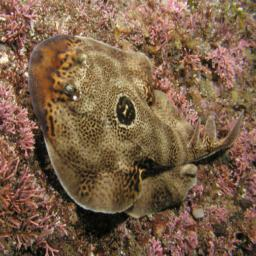
\includegraphics[width=0.8in]{n01496331_175_B} &
   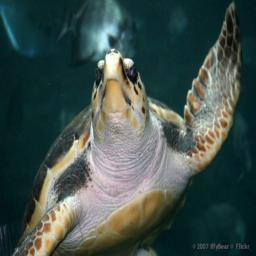
\includegraphics[width=0.8in]{n01664065_4022_B} &
   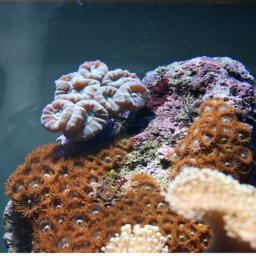
\includegraphics[width=0.8in]{n01917289_889_B} &
   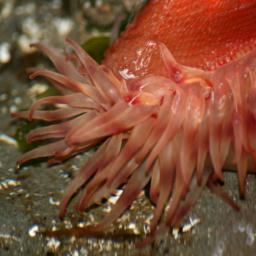
\includegraphics[width=0.8in]{n01914609_116_B} \\
   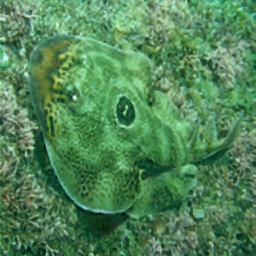
\includegraphics[width=0.8in]{n01496331_175_A} &
   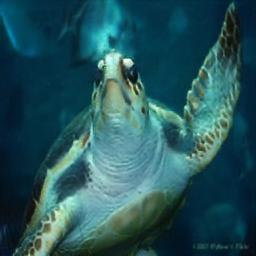
\includegraphics[width=0.8in]{n01664065_4022_A} &
   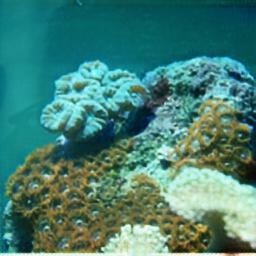
\includegraphics[width=0.8in]{n01917289_889_A} &
   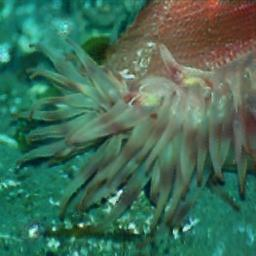
\includegraphics[width=0.8in]{n01914609_116_A} \\

\end{tabular}
\caption{Paired samples of ground truth and distorted images generated by CycleGAN. Top row: Ground truth.
Bottom row: Generated samples.}
\end{figure}


\begin{equation}
\begin{aligned}
   \min\limits_{G}\max\limits_{D} \mathbb{E} & _{I^C \sim p_{train}(I^C)} [logD(I^C)] + \\
   \mathbb{E} & _{I^D \sim p_{gen}(I^D)}[log(1 - D(G(I^D)))]
\end{aligned}
\end{equation}

\noindent Note for simplicity in notation, we will further omit $I^C \sim p_{train}$ and $I^D \sim p_{gen}$. In this formulation, the discriminator
is hypothesized as a classifier with a sigmoid cross entropy loss function,
which in practice may lead to issues such as the vanish gradient and mode collapse. There have been many recent works which
hypothesize a different loss function for the discriminator \cite{mao2016least,arjovsky2017wasserstein,gulrajani2017improved,zhao2016energy}.
We focus on the Wasserstein GAN (WGAN) \cite{arjovsky2017wasserstein} formulation, which proposes to use the Earth-Mover or \textit{Wasserstein-1}
distance $W$ by constructing a value function using the Kantorovich-Rubinstein duality \cite{villani2008optimal}. In this formulation, $W$ is
approximated given a set of $k$-Lipschitz functions $f$ modeled as neural networks. To ensure $f$ is $k$-Lipschitz, the weights of the discriminator
are clipped to some range $[-c, c]$. In our work, we adopt the Wasserstein GAN with gradient penalty (WGAN-GP) \cite{gulrajani2017improved}, which instead of
clipping network weights like in \cite{arjovsky2017wasserstein}, ensures the Lipschitz constraint by enforcing a soft constraint on the
gradient norm of the discriminator's output with respect to its input. Following \cite{gulrajani2017improved}, our new objective then becomes

\begin{equation}
\begin{aligned}
   \mathcal{L}_{WGAN}(G,D) = \mathbb{E} [D(I^C)] - \mathbb{E} & [D(G(I^D))] + \\
   \lambda \mathbb{E} & _{\hat{x} \sim \mathbb{P}_{\hat{x}}} [(|| \nabla_{\hat{x}} D(\hat{x})||_2 -1)^2 ],
\end{aligned}
\end{equation}

%\begin{equation}
%\begin{aligned}
%   \mathcal{L}_{GAN} = \mathbb{E}_{I^D \sim p_{gen}(I^D)} [D(I^D)] - \mathbb{E} & _{I^C \sim p_{train}(I^C)} [D(I^C)] + \\
%   \lambda \mathbb{E} & _{\hat{x} \sim \mathbb{P}_{\hat{x}}} [(|| \nabla_{\hat{x}} D(\hat{x})||_2 -1)^2 ].
%\end{aligned}
%\end{equation}

\noindent where $\mathbb{P}_{\hat{x}}$ is defined as samples along straight lines between pairs of points coming from the true data distribution
and the generator distribution, and $\lambda$ is a weighing factor. In order to give $G$ some sense of ground truth, we also consider the $L1$
loss

\begin{equation}
   \mathcal{L}_{L1} = \mathbb{E} [ || I^C - G(I^D) ||_1 ].
\end{equation}
%\begin{equation}
%   \mathcal{L}_{L1} = \mathbb{E}_{I^D \sim p_{gen}, I^C \sim p_{train}} [ || I^C - G(I^D) ||_1 ].
%\end{equation}

\noindent Combining these, we get our final objective function for our network, which we call Underwater GAN (UGAN),

\begin{equation}
   \begin{aligned}
      \mathcal{L}_{UGAN}^* = \min\limits_{G}\max\limits_{D} \mathcal{L}_{WGAN}(G,D) + \mathcal{L}_{L1}(G).
   \end{aligned}
\end{equation}


\subsection{Image Gradient Difference Loss}
Often times generative models produce blurry images. We explore a strategy to sharpen these predictions by
directly penalizing the differences of image gradient predictions in the generator, as proposed by \cite{mathieu2015deep}.
Given a ground truth image $I^C$, predicted image $I^P = G(I^C)$, and $\alpha \geq 1$, the Gradient Difference Loss (GDL) is given by

\begin{equation}
   \begin{aligned}
      \mathcal{L}_{GDL}(I^C, I^P) = \\ \sum\limits_{i,j} || & I^C_{i,j} - I^C_{i-1,j}| - | I^P_{i,j} - I^P_{i-1,j}||^{\alpha} + \\
      || & I^C_{i,j-1} - I^C_{i,j}| - | I^P_{i,j-1} - I^P_{i,j}||^{\alpha},
   \end{aligned}
\end{equation}

\noindent In our experiments, we denote our network as UGAN-P when considering the GDL, which can be expressed as

\begin{equation}
   \begin{aligned}
      \mathcal{L}_{UGAN}^* = \min\limits_{G}\max\limits_{D} \mathcal{L}_{WGAN}(G,D) + \mathcal{L}_{L1}(G) + \mathcal{L}_{GDL}
   \end{aligned}
\end{equation}


\subsection{Network Architecture and Training Details}
We use an encoder-decoder network similar to the work of \cite{isola2016image}, in which our generator is
structured as a ``U-Net'' \cite{ronneberger2015u} due to the structural similarity between input and output.
Encoder-decoder networks continuously downsample (encode) the input to a lower dimensional embedding, in which this embedding is then
upsampled (decode) to reconstruct the image. The advantage of using a ``U-Net'' comes from explicitly preserving spatial
dependencies produced by the encoder, as opposed to relying on the embedding to contain all of the information. This
is done by the addition of ``skip connections'', which concatenate the activations produced from a convolution
layer $i$ in the encoder to the input of a transpose convolution layer $n-i+1$ in the decoder, where $n$ is the
total number of layers in the network.

Our generator network can be viewed as two subnetworks, an encoder and a decoder. Each convolutional layer in the encoder and decoder
has a kernel size of 4 and stride 2. Following \cite{radford2015unsupervised}, we use Batch Normalization \cite{pmlr-v37-ioffe15}
except for the last layer of the decoder.

\footnote{Code is available at https://github.com/cameronfabbri/Underwater-Color-Correction}
L1 weight 100, batch size 32, wgan loss, learning rate 1e-4, IG weight 1.0 and 0.0, 100 epochs
Following WGAN-GP, the discriminator is updated $n$ times for every update of the generator, where $n = 5$.


\section{Experiments}

Here I want to show a number of things. First talk about the datasets used, Imagenet and the diving videos.
Second, show some general results. Explain how our network is able to do three very important things: 1) Restore an
image to its natural colors with varying amounts of distortion, i.e. blue hue, green hue, aka not just one type of
color distortion. 2) The network does not just subtract a certain hue from the entire image. Show how in the clownfish
image, part of the image has good colors, while part of it doesn't. Our network is able to leave correct colors. Third,
show that even images taken towards the water's surface, either above or below, are able to be restored correctly.

Third mention that since CycleGAN has a cycle consistent nature, compare their results. Then from there go into how
ours are better by showing results from Canny Edge Detector.


\begin{figure}
\centering
\begin{tabular}{p{1.7cm} p{1.7cm} p{1.7cm} p{1.5cm}}
   % TODO 
   % I couldn't figure out how to get the text centered above the images
   % Also, the numbers below the images should be centered too, and more
   % obviously below the row instead of seemlingly above the next one. Those
   % numbers are the distances in pixel space (normalized between [0,1]) from
   % the edge image to the original edge image.


   \small{Original} & \small{CycleGAN} & \small{UGAN} & \small{UGAN-P} \\

   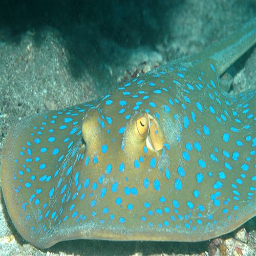
\includegraphics[width=0.8in]{n01496331_15872_original} &
   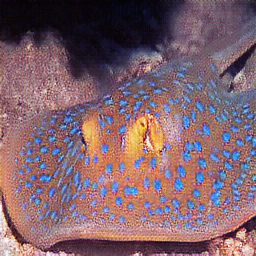
\includegraphics[width=0.8in]{n01496331_15872_cimg}     &
   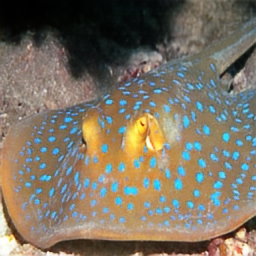
\includegraphics[width=0.8in]{n01496331_15872_u0img}    &
   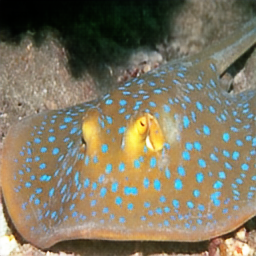
\includegraphics[width=0.8in]{n01496331_15872_u1img}    \\ [-1ex]
   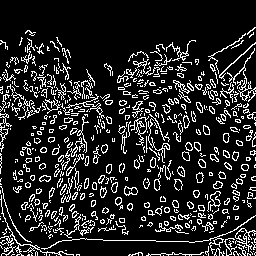
\includegraphics[width=0.8in]{n01496331_15872_oedges}   &
   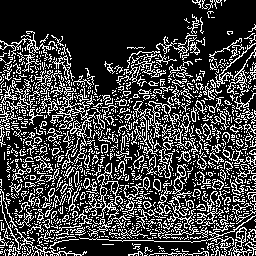
\includegraphics[width=0.8in]{n01496331_15872_cedges}   &
   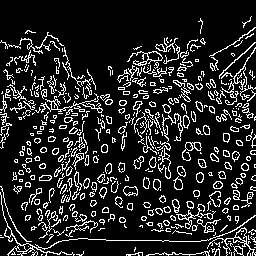
\includegraphics[width=0.8in]{n01496331_15872_u0edges}  &
   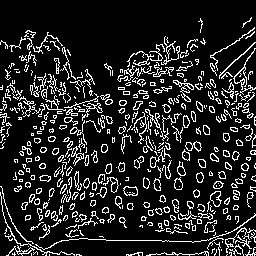
\includegraphics[width=0.8in]{n01496331_15872_u1edges}  \\
   0 & \small{125.78} & \small{80.68} & \small{78.49} \\

   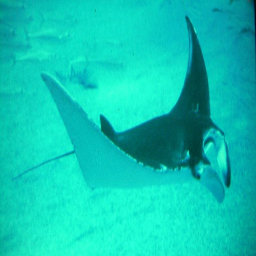
\includegraphics[width=0.8in]{n01496331_22079_original} &
   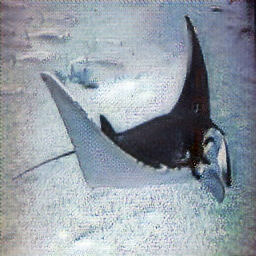
\includegraphics[width=0.8in]{n01496331_22079_cimg}     & 
   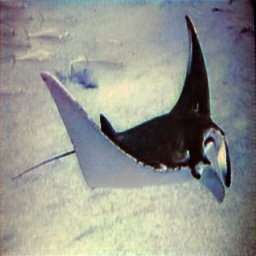
\includegraphics[width=0.8in]{n01496331_22079_u0img}    &
   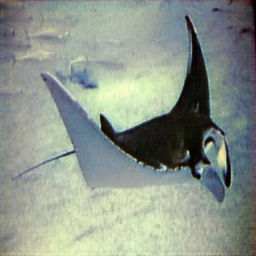
\includegraphics[width=0.8in]{n01496331_22079_u1img}    \\ [-1ex]
   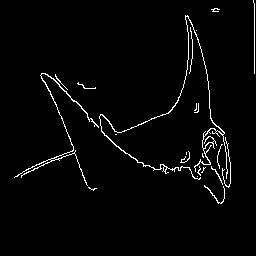
\includegraphics[width=0.8in]{n01496331_22079_oedges}   &
   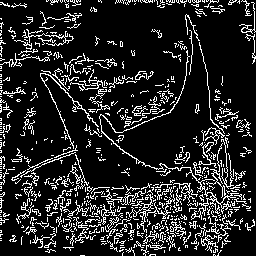
\includegraphics[width=0.8in]{n01496331_22079_cedges}   &
   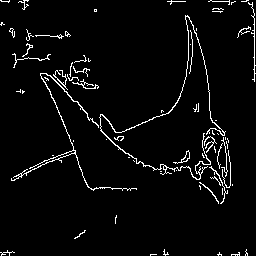
\includegraphics[width=0.8in]{n01496331_22079_u0edges}  &
   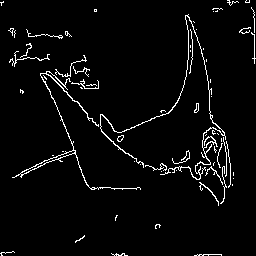
\includegraphics[width=0.8in]{n01496331_22079_u1edges}  \\
   0 & \small{94.57} & \small{38.22} & \small{37.29} \\

   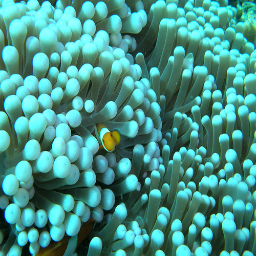
\includegraphics[width=0.8in]{n02607072_4739_original} &
   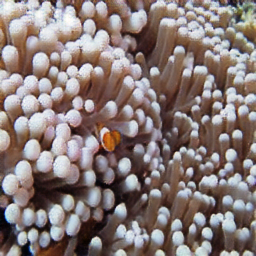
\includegraphics[width=0.8in]{n02607072_4739_cimg} &
   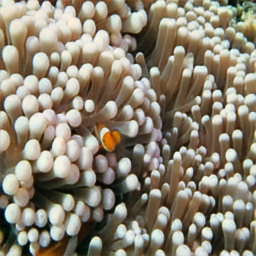
\includegraphics[width=0.8in]{n02607072_4739_u0img} &
   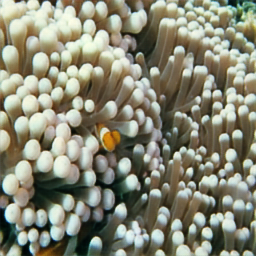
\includegraphics[width=0.8in]{n02607072_4739_u1img} \\ [-1ex]
   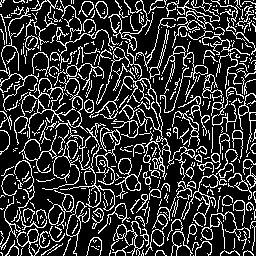
\includegraphics[width=0.8in]{n02607072_4739_oedges} &
   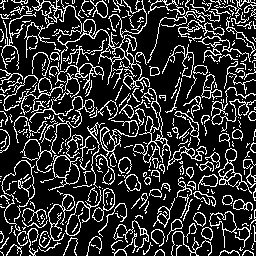
\includegraphics[width=0.8in]{n02607072_4739_cedges} &
   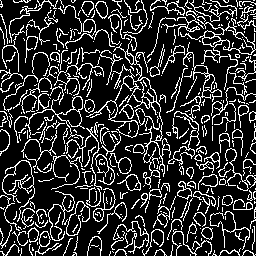
\includegraphics[width=0.8in]{n02607072_4739_u0edges} &
   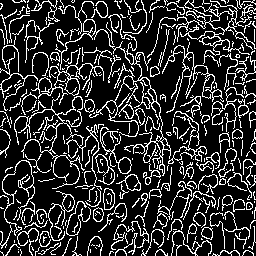
\includegraphics[width=0.8in]{n02607072_4739_u1edges} \\
   0 & \small{100.69} & \small{87.81} & \small{87.95} \\
   
\end{tabular}
\caption{Running the Canny Edge Detector on sample images. Both variants of UGAN contain less noise than CycleGAN,
and are closer in the image space to the original. For each pair, the top row is the input image, and bottom row
the result of the edge detector.}
\end{figure}


\section{Conclusion}



\section*{Acknowledgment}

%
%\begin{thebibliography}{1}
%\bibitem{hires}{Johnson‐Roberson, Matthew, et al. "High‐Resolution Underwater Robotic Vision‐Based Mapping and Three‐Dimensional Reconstruction for Archaeology." Journal of Field Robotics 34.4 (2017): 625-643.}
%
%\bibitem{col1}{Zhang, Richard, Phillip Isola, and Alexei A. Efros. "Colorful image colorization." European Conference on Computer Vision. Springer International Publishing, 2016.}

%\bibitem{col2}{Cheng, Zezhou, Qingxiong Yang, and Bin Sheng. "Deep colorization." Proceedings of the IEEE International Conference on Computer Vision. 2015.}

%\bibitem{col3}{Iizuka, Satoshi, Edgar Simo-Serra, and Hiroshi Ishikawa. "Let there be color!: joint end-to-end learning of global and local image priors for automatic image colorization with simultaneous classification." ACM Transactions on Graphics (TOG) 35.4 (2016): 110.}

%\bibitem{pix2pix}{Isola, Phillip, et al. "Image-to-image translation with conditional adversarial networks." arXiv preprint arXiv:1611.07004 (2016).}

%\bibitem{watergan}{Li, Jie, et al. "WaterGAN: Unsupervised Generative Network to Enable Real-time Color Correction of Monocular Underwater Images." arXiv preprint arXiv:1702.07392 (2017).}

%\end{thebibliography}

%\bibliography{/home/fabbric/Research/colorCorrection/files/paper/cambibs}
\bibliography{cambibs}
\bibliographystyle{ieeetr}

% that's all folks
\end{document}


